\clearpage
%%=========================================
% Den litt rare section-formuleringen er for å en kortere header-tittel siden den er for lang ellers.
% \sectionmark{} inne i {section title as seen in paper ...} er for å få riktig header der en section begynner på en oddetallsside.
%
%   \section[section title as seen in TOC]{section title as seen in paper%
%       \sectionmark{section title as seen in header}}\sectionmark{section title as seen in header}
%
%\section[Surface Analysis of Substrate A with Surface Pre-Growth Preparation]{Surface Analysis of Substrate A with Surface Pre-Growth Preparation%
%    \sectionmark{Surface Analysis of Pre-Growth Substrate A}}\sectionmark{Surface Analysis of Pre-Growth Substrate A}\label{sec:subAb}
    
\section{Surface Analysis of Substrate A after Etching}
As substrate A was already polished by the vendor, the surface pre-growth preparation simply consisted of a \ce{Br}:methanol etch. The dark field images taken of substrate A after etching showed that the etch had left more particles on the surface than before, compare Fig.~\ref{fig:subAa_om_df} and Fig.~\ref{fig:subAb_om_df}. The density of particles and features larger than \SI{0.5}{\micro\metre} had increased from \SI{\sim 4e2}{\centi\metre^{-2}} to \SI{\sim 1e3}{\centi\metre^{-2}} close to the centre of the substrate. %\todo{Bare etsing får til flere partikler? Hvor kommer de fra? Løsnet fra kantene og løst seg i esevæsken for så å falle ned. settle on the substrate surface. }

\begin{figure}[htbp]
    \centering
    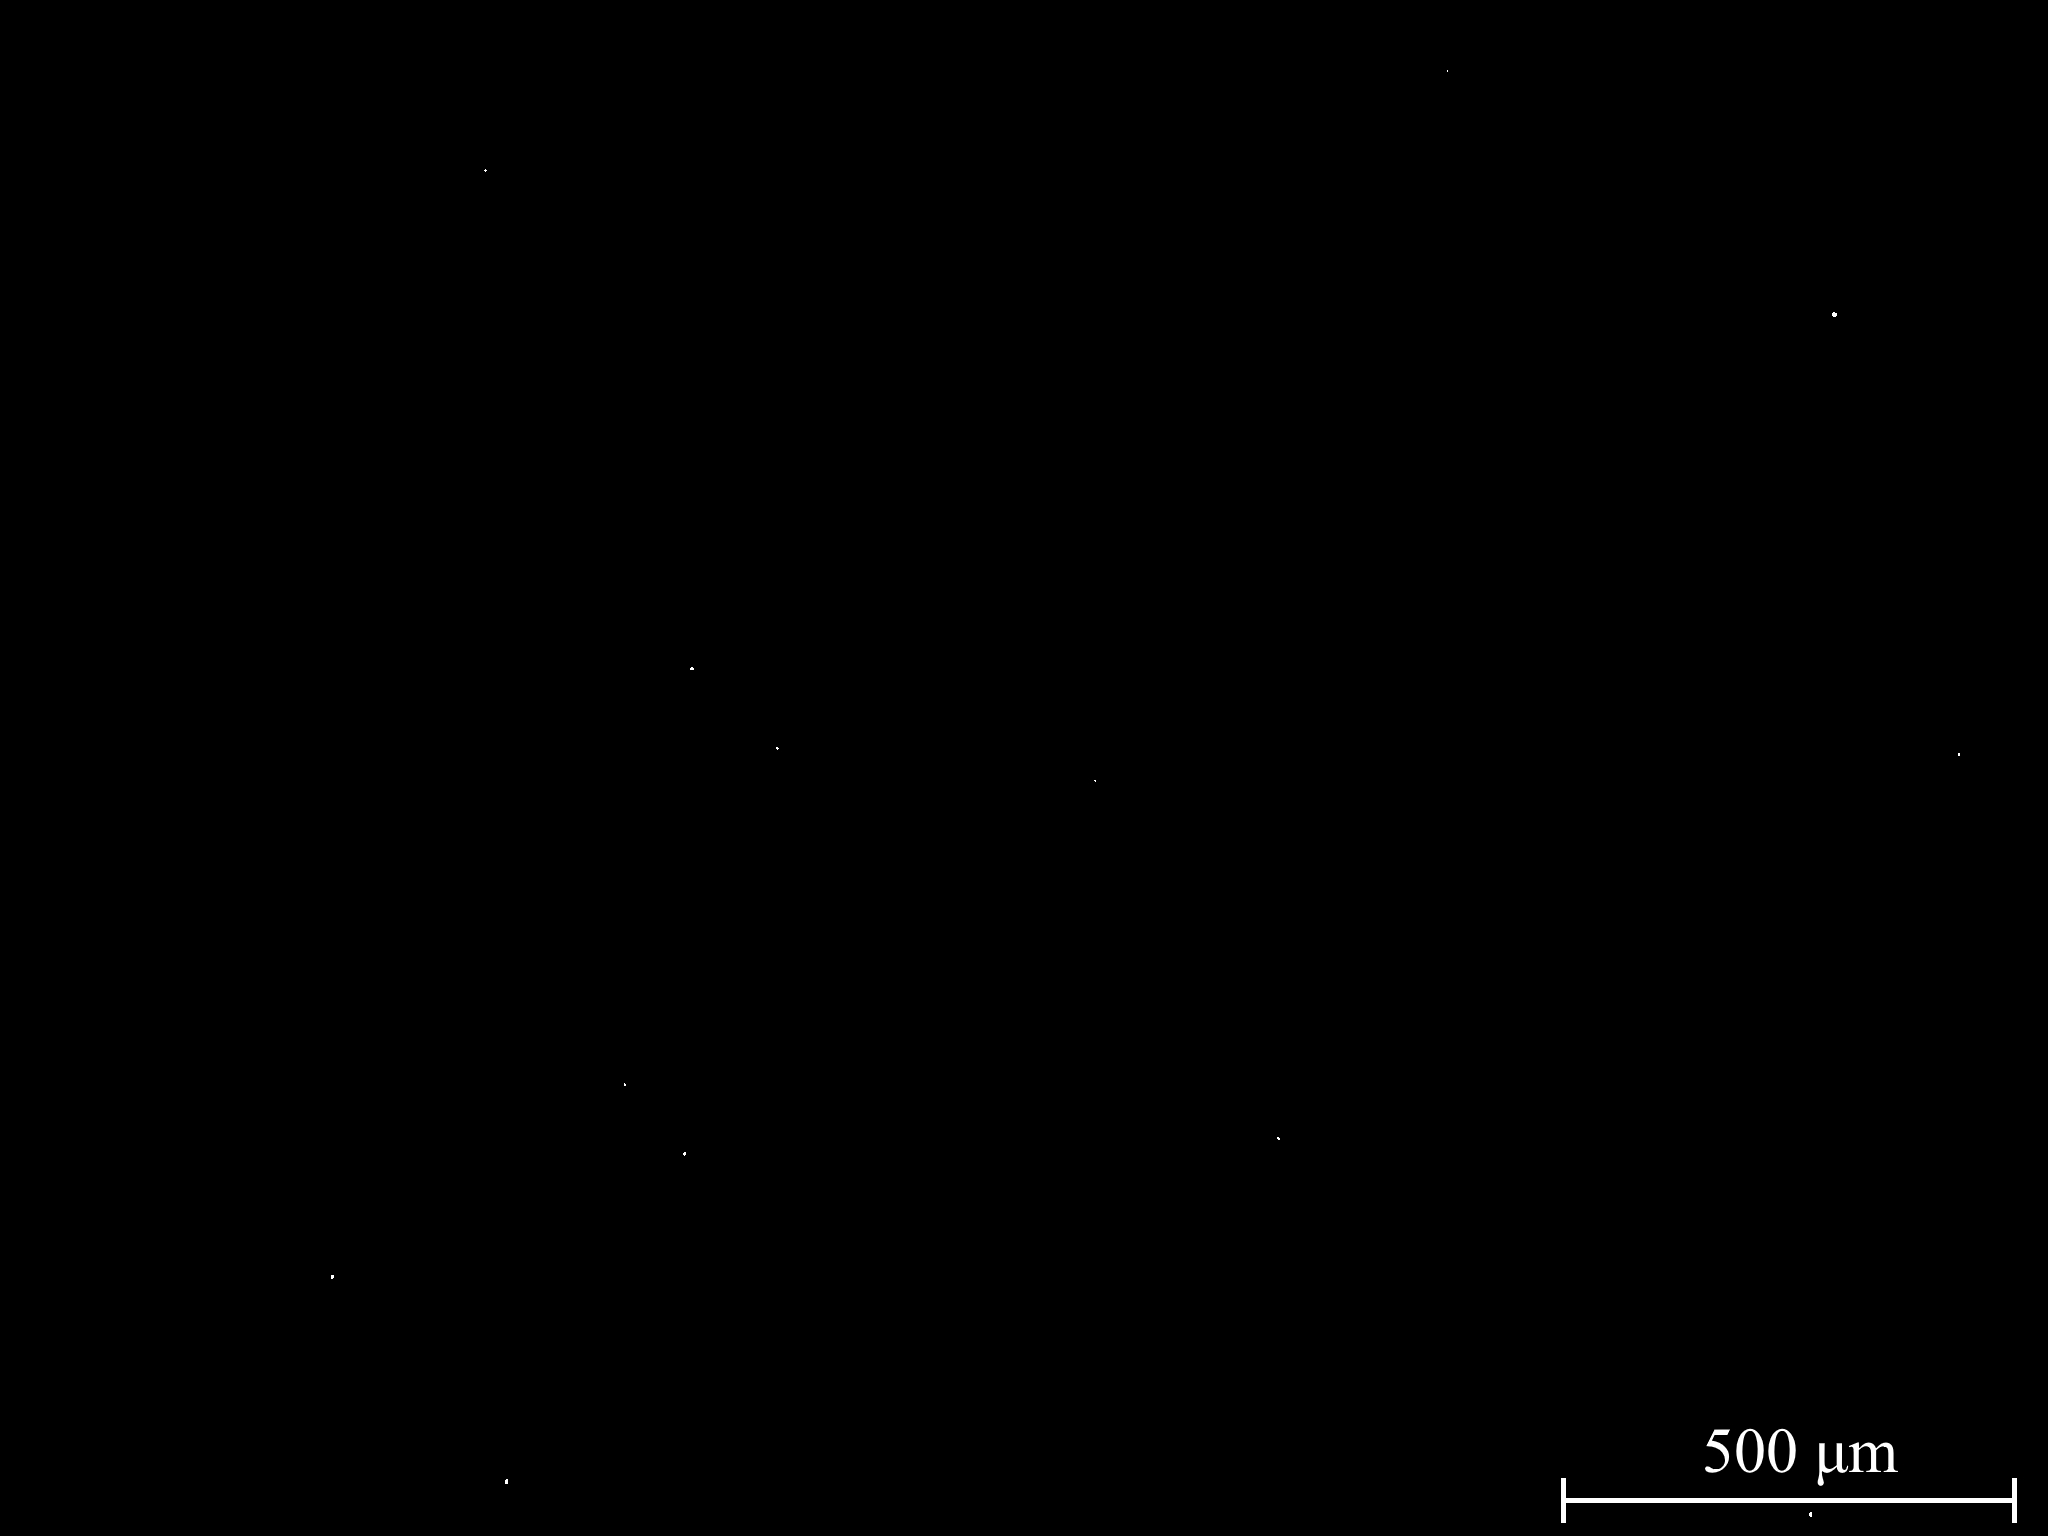
\includegraphics[width=\linewidth]{subAb_om_df_n021.jpg}
    \caption[Dark field optical microscopy image of substrate A after a \ce{Br}:methanol etch.]{Dark field optical microscopy image of substrate A after a \ce{Br}:methanol etch taken near the centre of the substrate.}\label{fig:subAb_om_df}
\end{figure}

\Ac{sem} shows the surface at a higher magnification and it revealed that there were much smaller particles distributed over the surface as well. Whereas it was difficult to focus the \ac{sem} beam at the surface of the as-received substrate, after etch this was not a problem due to the higher density of particles. There were a higher density of particles near the edges and corners of the substrate than in the centre, as can be seen in Fig.~\ref{fig:subAb_sem_typical_centre} and Fig.~\ref{fig:subAb_sem_typical_edge} respectively.

\begin{figure}[htbp]
    \mySubfigure{0.49\textwidth}{subAb_sem_02b_m008.png}[fig:subAb_sem_typical_centre]
    \hfill
    \mySubfigure{0.49\textwidth}{subAb_sem_02a_m004.png}[fig:subAb_sem_typical_edge]
    \caption[\Ac{sem} images of typical areas on substrate A after a \ce{Br}:methanol etch.]{\Ac{sem} images of \subref{fig:subAb_sem_typical_centre} a typical area near the centre and \subref{fig:subAb_sem_typical_edge} an area with a high density of particles near the edge of substrate A after a \ce{Br}:methanol etch.}\label{fig:subAb_sem_typical}
\end{figure}

%%=========================================
\subsection{Particles}
Four different types of particles were found on the surface of substrate A after a \ce{Br}:methanol etch, see Fig.~\ref{fig:subAb_sem_w_eds}.

\begin{figure}[htbp]
    \centering
    \begin{subfigure}[t]{\textwidth}
        \caption{}\label{fig:subAb_silica}
          \begin{minipage}[c]{0.43\linewidth}
            \centering
            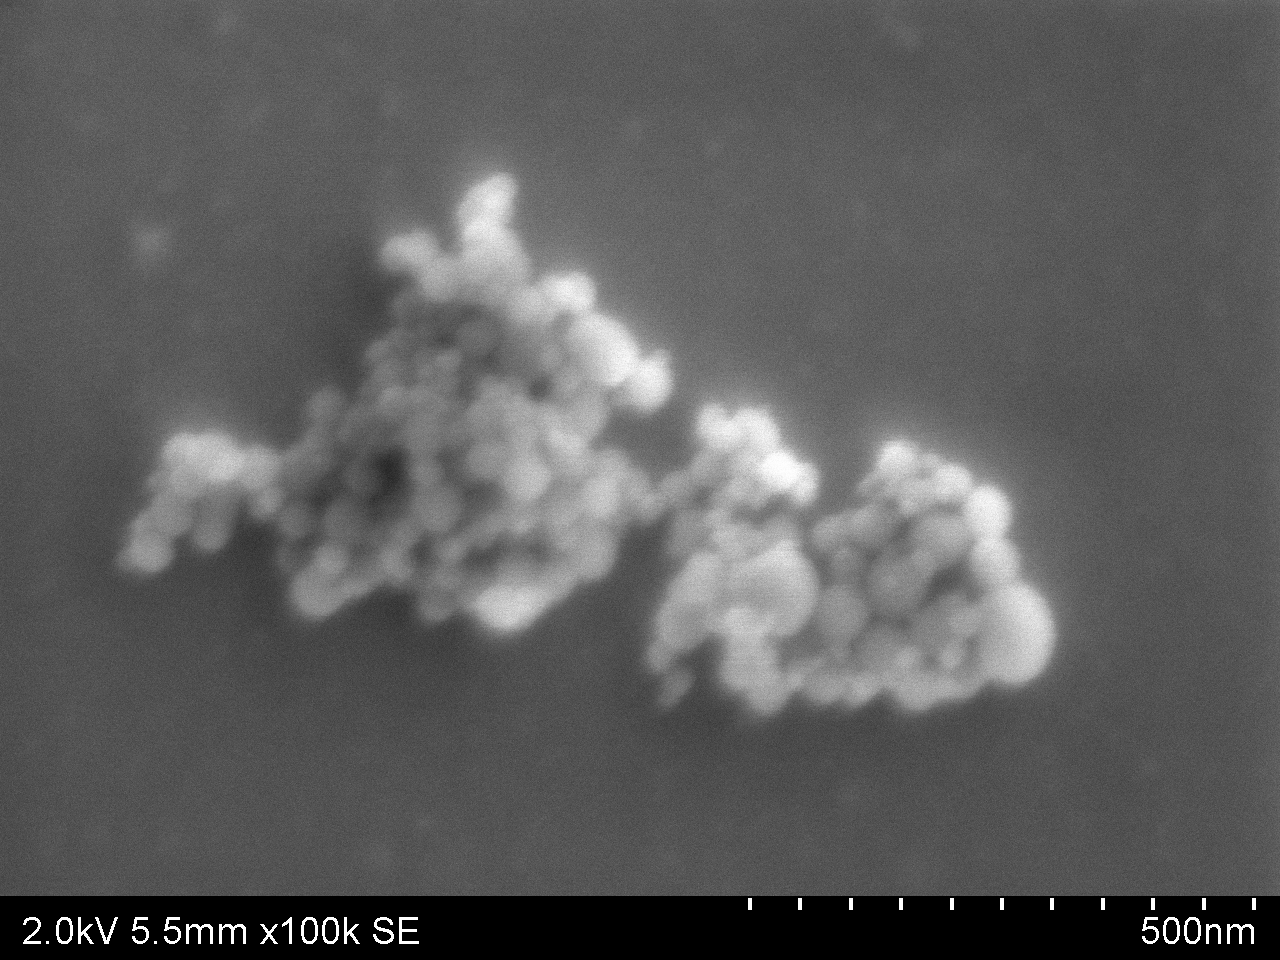
\includegraphics[width=\linewidth]{subAb_sem_03_m004.png}
          \end{minipage}
          \hfill
          \begin{minipage}[c]{0.43\linewidth}
            \centering
            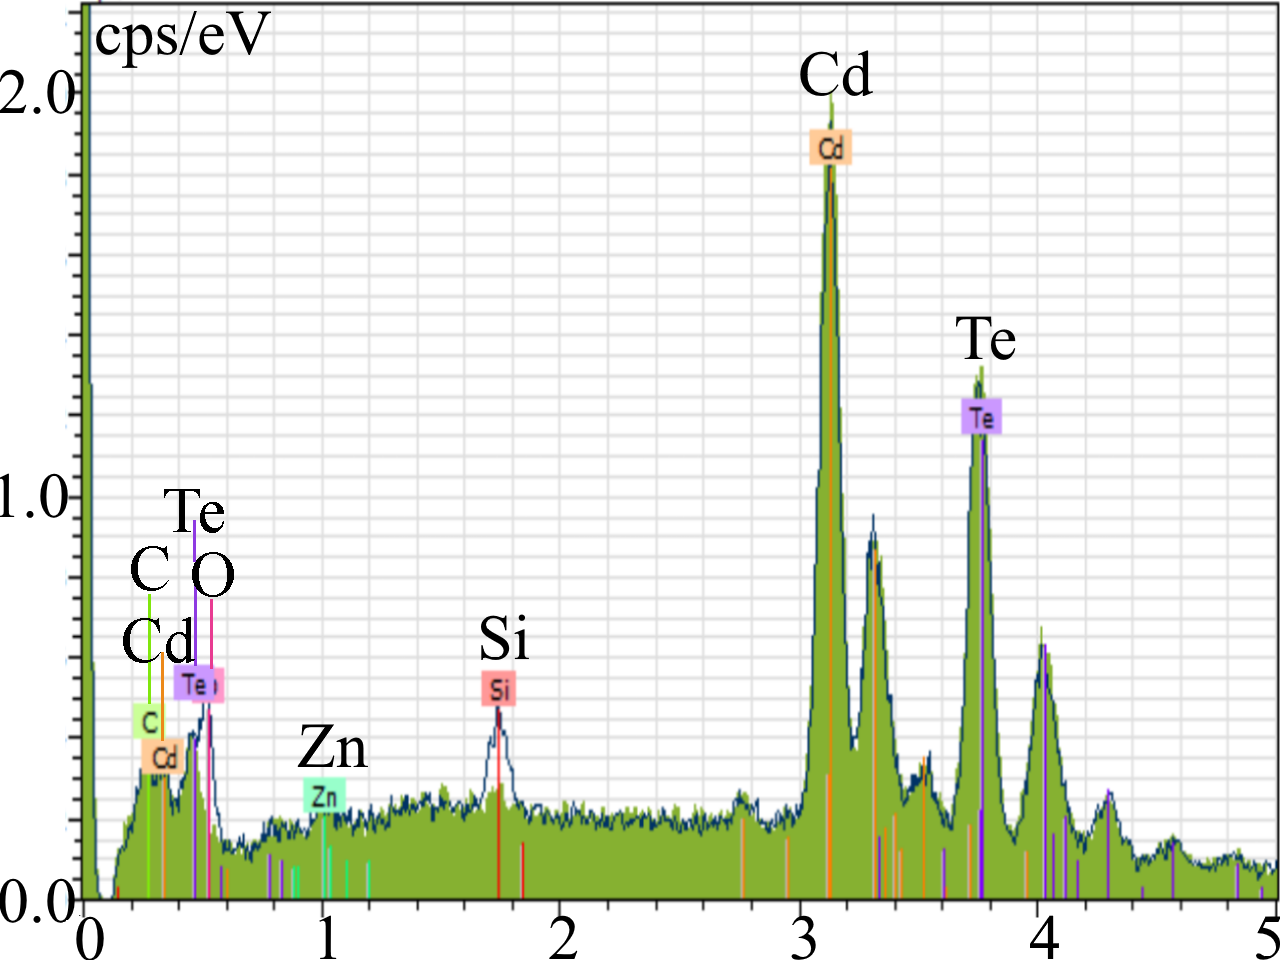
\includegraphics[width=\linewidth]{subAb_eds_03_m004.png}
          \end{minipage}
          \begin{minipage}[c]{0.11\linewidth}
            \centering
            \atomicTable[\ce{Te}&\SI{39.21}{}][\ce{Cd}&\SI{37.98}{}][\ce{O}&\SI{11.45}{}][\ce{Si}&\SI{5.74}{}][\ce{C}&\SI{4.19}{}][\ce{Zn}&\SI{1.42}{}]%OK
          \end{minipage}
    \end{subfigure}
    \par\bigskip
    \begin{subfigure}[t]{\textwidth}
        \caption{}\label{fig:subAb_silica2}
          \begin{minipage}[c]{0.43\linewidth}
            \centering
            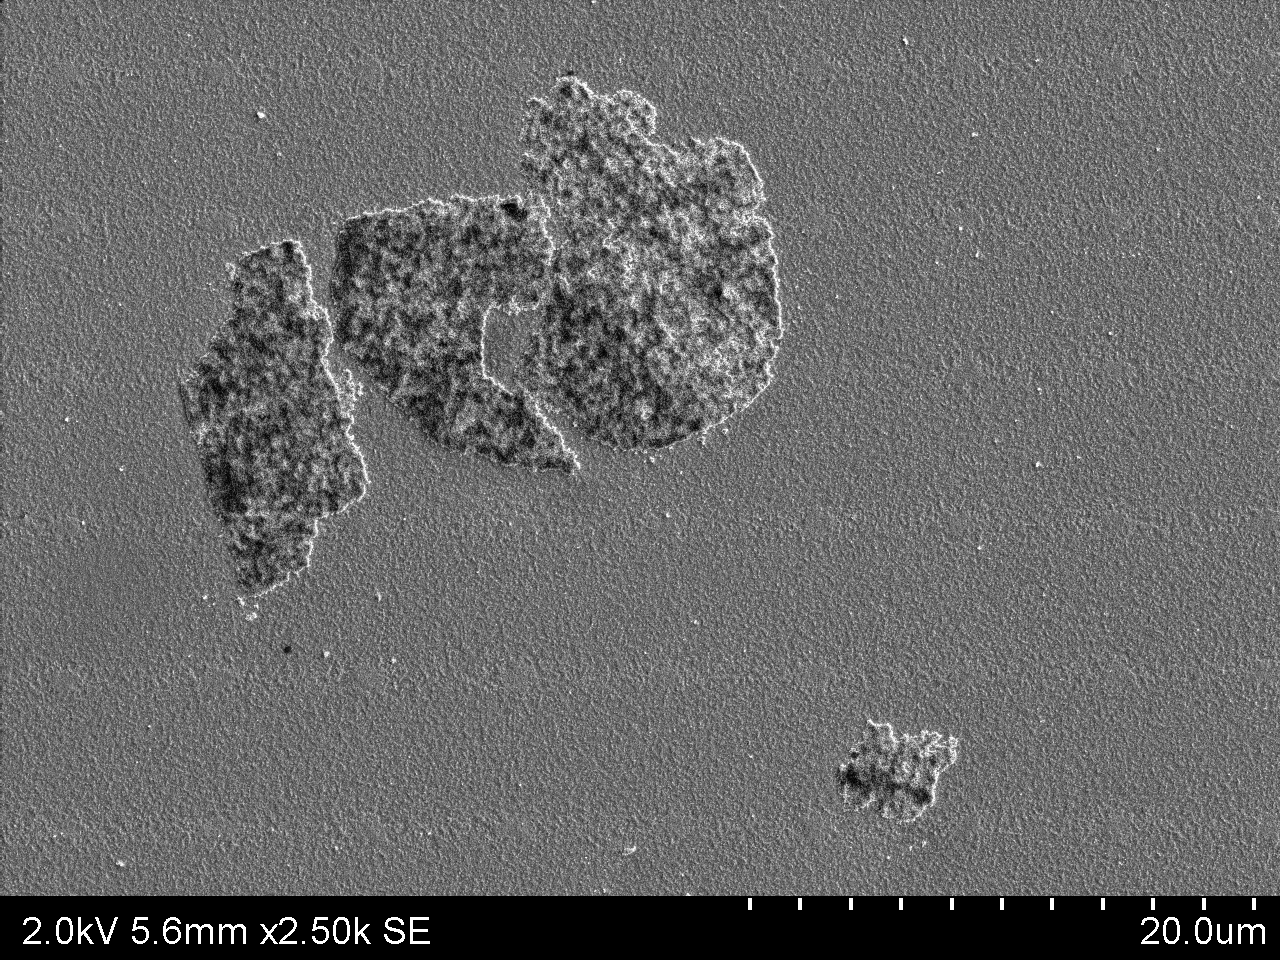
\includegraphics[width=\linewidth]{subAb_sem_03_m005.png}
          \end{minipage}
          \hfill
          \begin{minipage}[c]{0.43\linewidth}
            \centering
            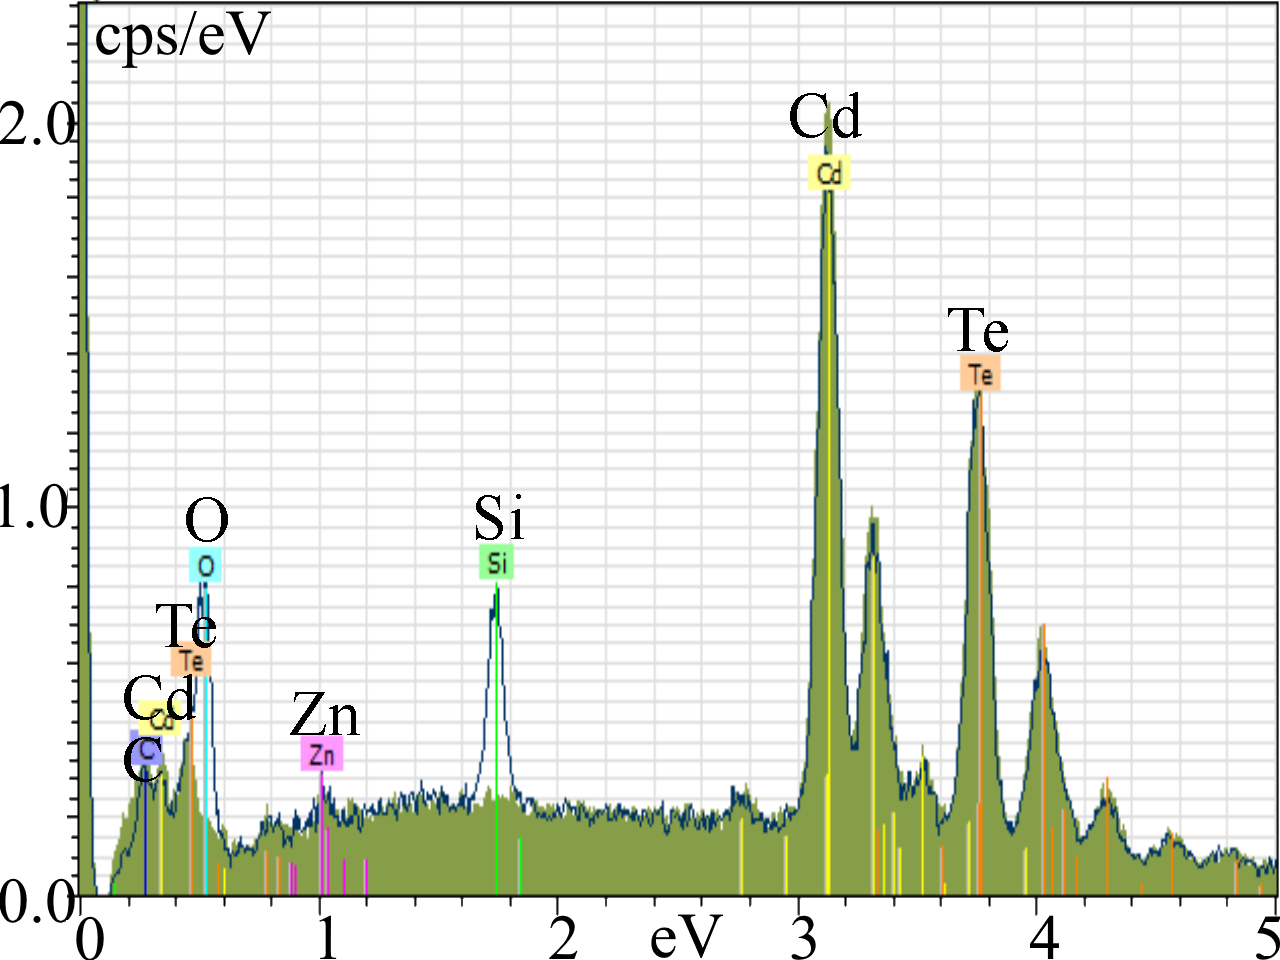
\includegraphics[width=\linewidth]{subAb_eds_03_m005.png}
          \end{minipage}
          \begin{minipage}[c]{0.11\linewidth}
            \centering
            \atomicTable[\ce{Te}&\SI{32.56}{}][\ce{Cd}&\SI{32.17}{}][\ce{O}&\SI{20.07}{}][\ce{Si}&\SI{11.13}{}][\ce{C}&\SI{3.00}{}][\ce{Zn}&\SI{1.07}{}]%OK
          \end{minipage}
    \end{subfigure}
    \par\bigskip
    \begin{subfigure}[t]{\textwidth}
        \caption{}\label{fig:subAb_br-stain}
          \begin{minipage}[c]{0.43\linewidth}
            \centering
            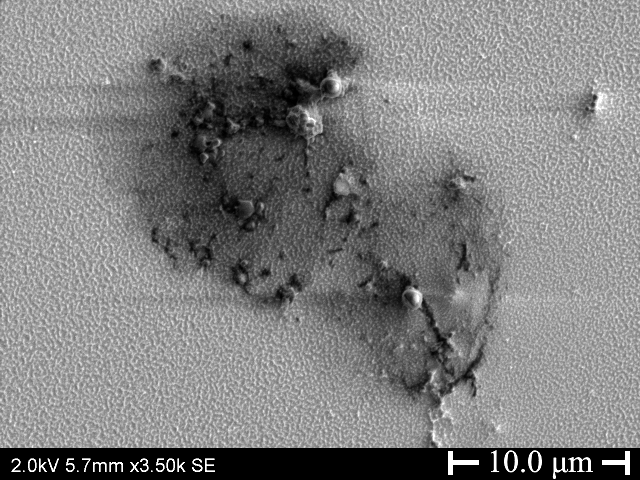
\includegraphics[width=\linewidth]{subAb_sem_03_m011.png}
          \end{minipage}
          \hfill
          \begin{minipage}[c]{0.43\linewidth}
            \centering
            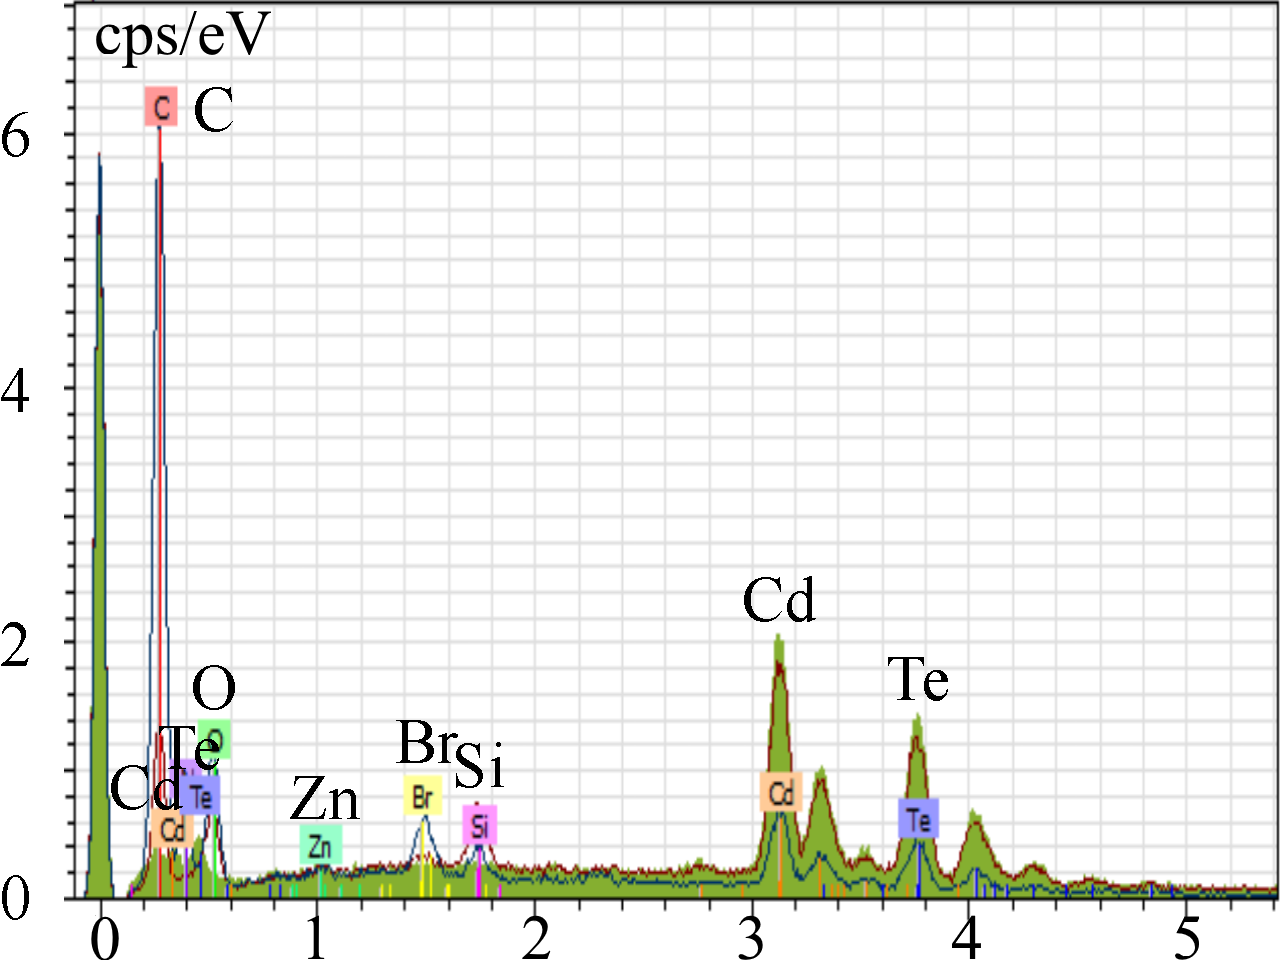
\includegraphics[width=\linewidth]{subAb_eds_03_m011.png}
          \end{minipage}
          \begin{minipage}[c]{0.11\linewidth}
            \centering
            \atomicTable[\ce{C}&\SI{61.19}{}][\ce{N}&\SI{13.84}{}][\ce{O}&\SI{13.51}{}][\ce{Cd}&\SI{4.11}{}][\ce{Te}&\SI{3.64}{}][\ce{Si}&\SI{1.60}{}][\ce{Br}&\SI{1.46}{}][\ce{S}&\SI{0.38}{}][\ce{Zn}&\SI{0.27}{}]
          \end{minipage}
    \end{subfigure}
    \caption[\Ac{sem} images, \ac{eds} spectra, and \ac{eds} atomic compositions of three different types of particles and one type of stain found on substrate A after a \ce{Br}:methanol etch.]{High resolution \ac{sem} images of four different types of particles and one stain found on substrate A after a \ce{Br}:methanol etch and the corresponding \ac{eds} spectra and atomic compositions: \subref{fig:subAb_silica} Silica (\ce{SiO2}) polishing grit agglomeration; \subref{fig:subAb_silica2} silica (\ce{SiO2}) particles; \subref{fig:subAb_br-stain} stain consisting of bromine, carbon, and oxygen; and \subref{fig:subAb_br-particle} particle consisting of bromine, carbon, and oxygen. The blue line represents the \ac{eds} spectrum of the particle, while the filled green represents the \ac{eds} spectrum of the underlying substrate.}\label{fig:subAb_sem_w_eds}
\end{figure}
%
\begin{figure}[htbp]
\ContinuedFloat
    \centering
    \begin{subfigure}[t]{\textwidth}
        \caption{}\label{fig:subAb_br-particle}
          \begin{minipage}[c]{0.43\linewidth}
            \centering
            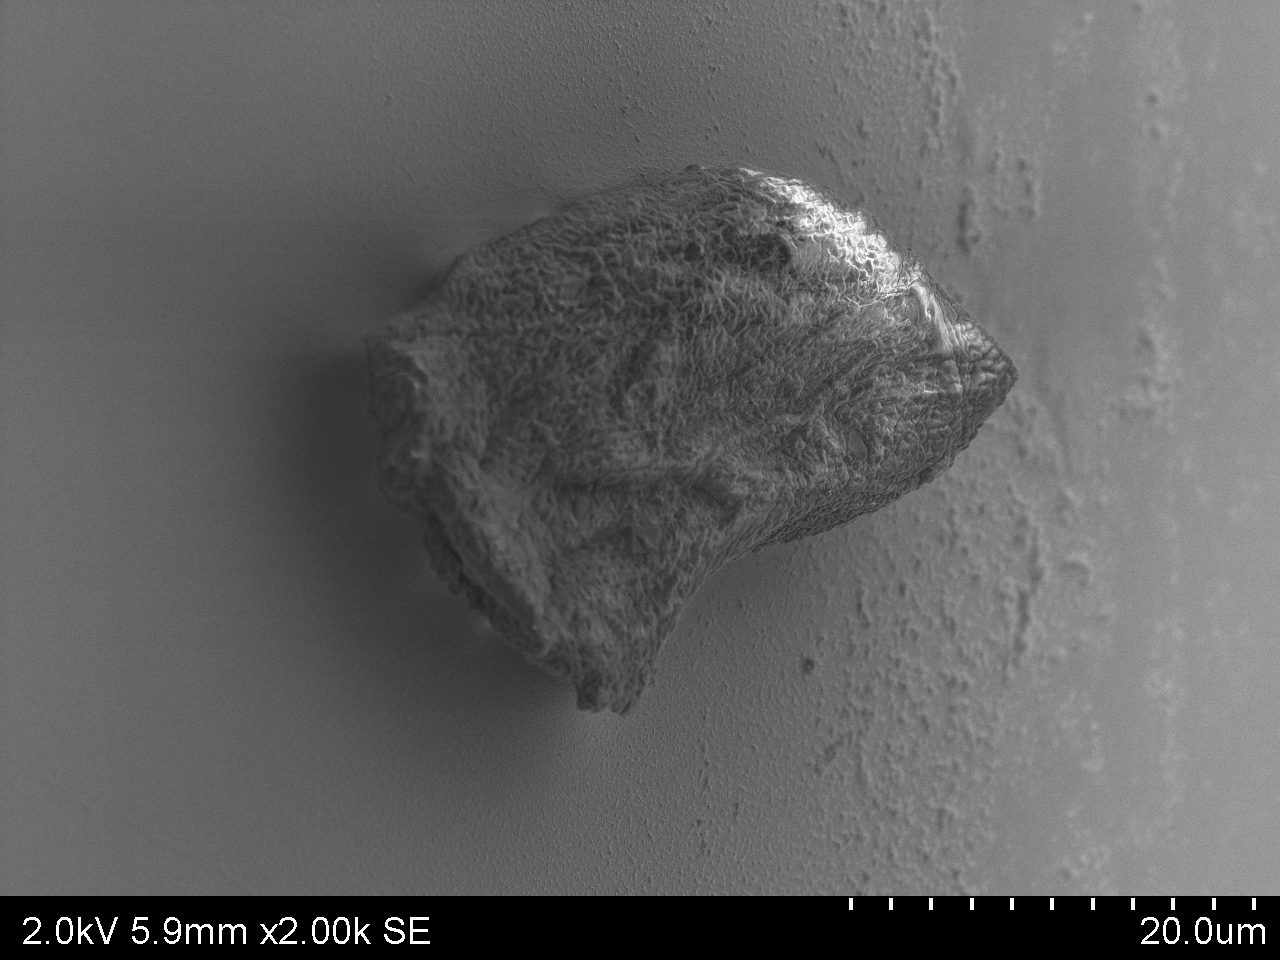
\includegraphics[width=\linewidth]{subAb_sem_03_m013.png}
          \end{minipage}
          \hfill
          \begin{minipage}[c]{0.43\linewidth}
            \centering
            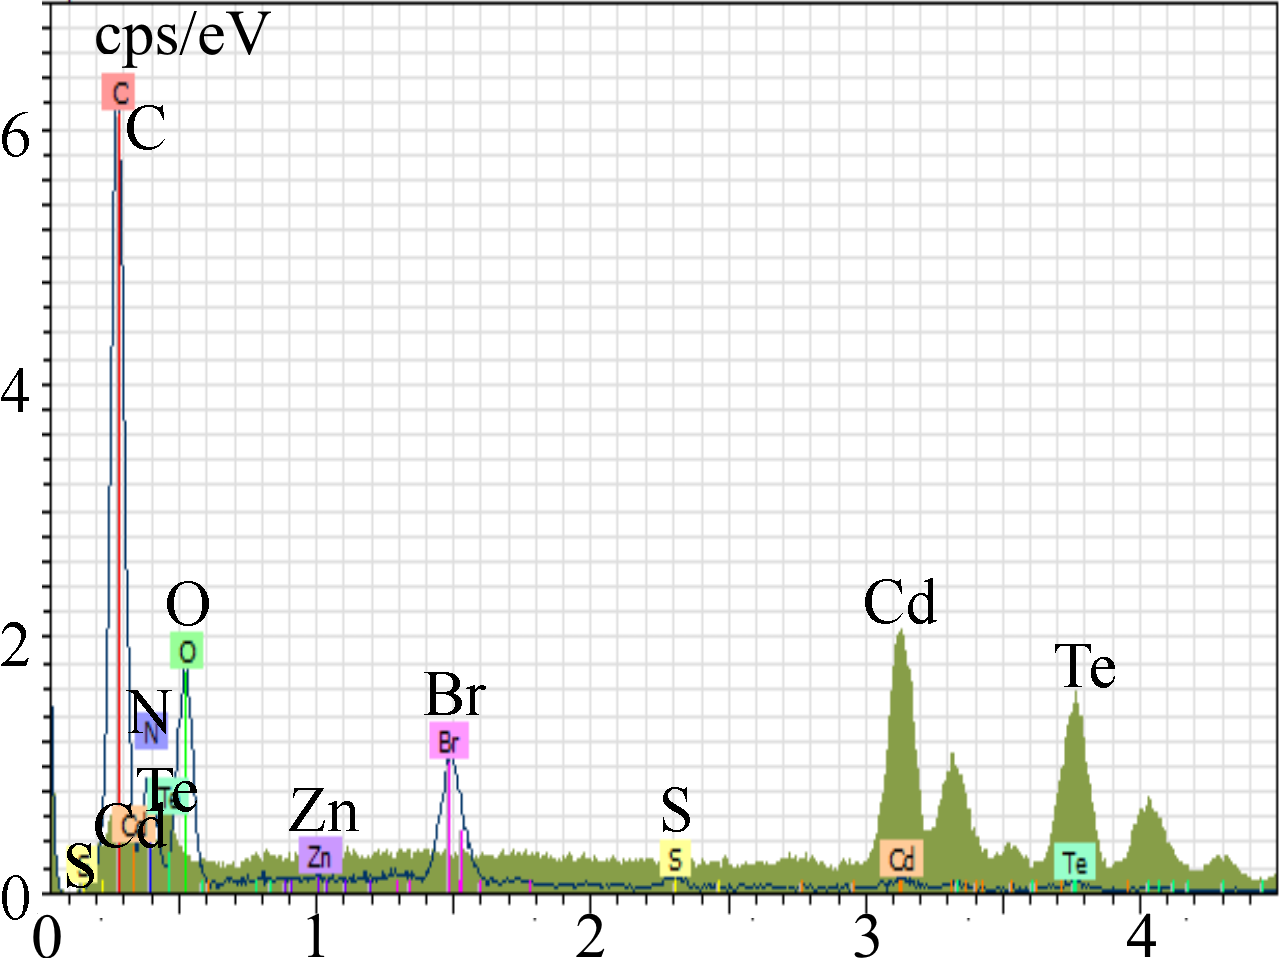
\includegraphics[width=\linewidth]{subAb_eds_03_m013.png}
          \end{minipage}
          \begin{minipage}[c]{0.11\linewidth}
            \centering
            \atomicTable[\ce{C}&\SI{59.19}{}][\ce{O}&\SI{18.86}{}][\ce{N}&\SI{18.63}{}][\ce{Br}&\SI{2.15}{}][\ce{Te}&\SI{0.41}{}][\ce{Cd}&\SI{0.37}{}][\ce{S}&\SI{0.35}{}][\ce{Zn}&\SI{0.04}{}]
          \end{minipage}
    \end{subfigure}
    \captionsetup{list=no}
    \caption{\emph{(continued)}}
\end{figure}


\subsubsection{Silica (\ce{SiO2}) polishing grit and agglomeration}

Silica polishing grit were found on the surface of the substrate after \ce{Br}:methanol etch, see Fig.~\ref{fig:subAb_silica}. The grit density was higher and there were larger agglomerations of grit than before the etch. Silica grit particles are not used at the Epitek laboratory, and hence, it is believed that the source of the particles must be the substrate itself. \Ac{sem} images of the edge of the as-received substrate A showed that there were a layer of something brighter than the substrate on the bevelled edges, possibly a lot of grit particles, see Fig.~\ref{fig:subAa_corner_w_grit}. The polishing grit may have originated from the bevelled edges or from underneath the as-received substrate, and been distributed over the surface during the preparation etch procedure. There is a slight possibility that the particles came from the beaker where the substrate was etched because the same beaker was used for the polished substrate B, but that is not very likely. The reason the increase in particles after etch has not been detected earlier is that \ac{lpe} is somewhat forgiving of impurities on the surface as there is a period of surface melting before the film starts to grow. Nevertheless, it will most likely influence the film quality and the bevelled edges and the backside of the substrate have to be studied further in future studies.

\begin{figure}[htbp]
    \centering
    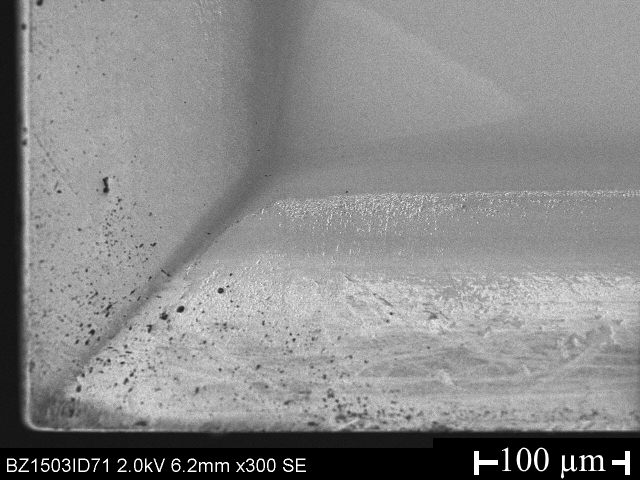
\includegraphics[width=0.7\linewidth]{SEM_BZ1503A_b_m013.png}
    \caption{\Ac{sem} image of the corner of the as-received substrate A.}
    \label{fig:subAa_corner_w_grit}
\end{figure}

The silica polishing grit observed in \ac{sem} were found all over the surface. The particle density was found to be between \SI{2e+05}{\centi\metre^{-2}} and \SI{1e+07}{\centi\metre^{-2}}. The average particle density was \SI{2e+06}{\centi\metre^{-2}} with a standard deviation of \SI{3e+06}{\centi\metre^{-2}}. A graphical representation of the particle density at different locations on substrate A can be seen in Fig.~\ref{fig:subAb_densityData}. There was a tendency of higher density towards the edges and corners.

\begin{figure}[htbp]
    \centering
    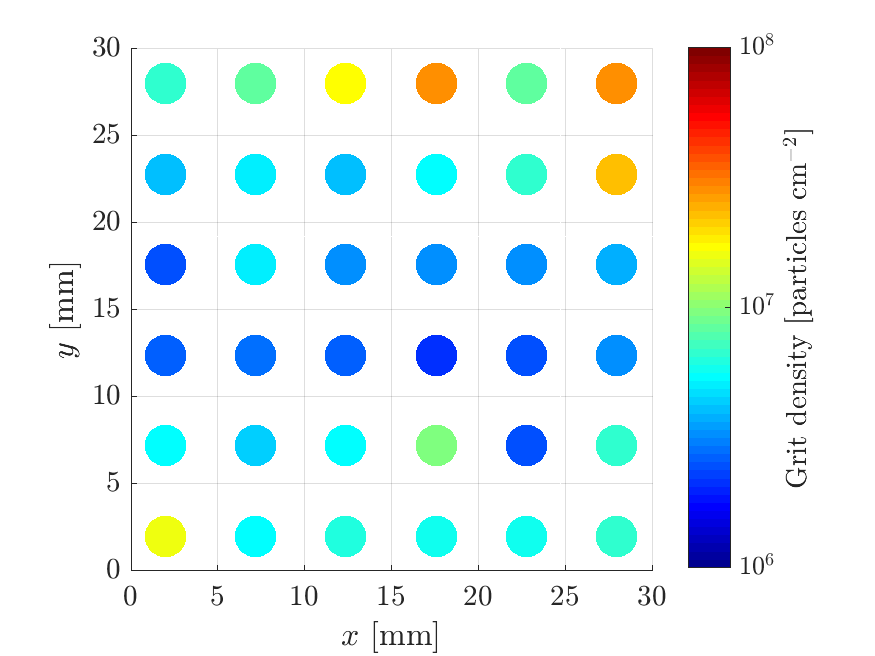
\includegraphics[width=0.5\linewidth]{subAb_densityData.png}
    \caption[Map of the polishing grit density on substrate A after a \ce{Br}:methanol etch.]{A map of the polishing grit density at 36 different locations on the $\SI{30}{\milli\metre}\times\SI{30}{\milli\metre}$ substrate A after a \ce{Br}:methanol etch. The density measurements were obtained by counting the number of polishing grits in \ac{sem} images covering $\SI{25.4}{\micro\metre}\times\SI{17.8}{\micro\metre}$ areas. In total, \SI{0.002}{\percent} of the substrate surface was measured. The polishing grit density was observed to vary between \SI{2e+05}{\centi\metre^{-2}} and \SI{1e+07}{\centi\metre^{-2}}. The empty grid points represent where the density was less than the detection limit of \SI{2e+5}{\centi\metre^{-2}}.}
    \label{fig:subAb_densityData}
\end{figure}

Fig.~\ref{fig:subAb_silica2} shows four particles ranging from \SI{4}{\micro\metre} to \SI{15}{\micro\metre} in size. These particles consist of \ce{SiO2}. When looking at the particles at higher magnification, see Fig.~\ref{fig:subAb_silica2_magnified}, they appeared to be made up of smaller, circular particles with a diameter of \SIrange{50}{100}{\nano\metre}. Clearly, silica polishing grit had accumulated to a larger structure. These structures were mainly observed close to the edges of the substrate and could be originating from the suspected layer of polishing grit on the bevelled edges.

\begin{figure}
    \centering
    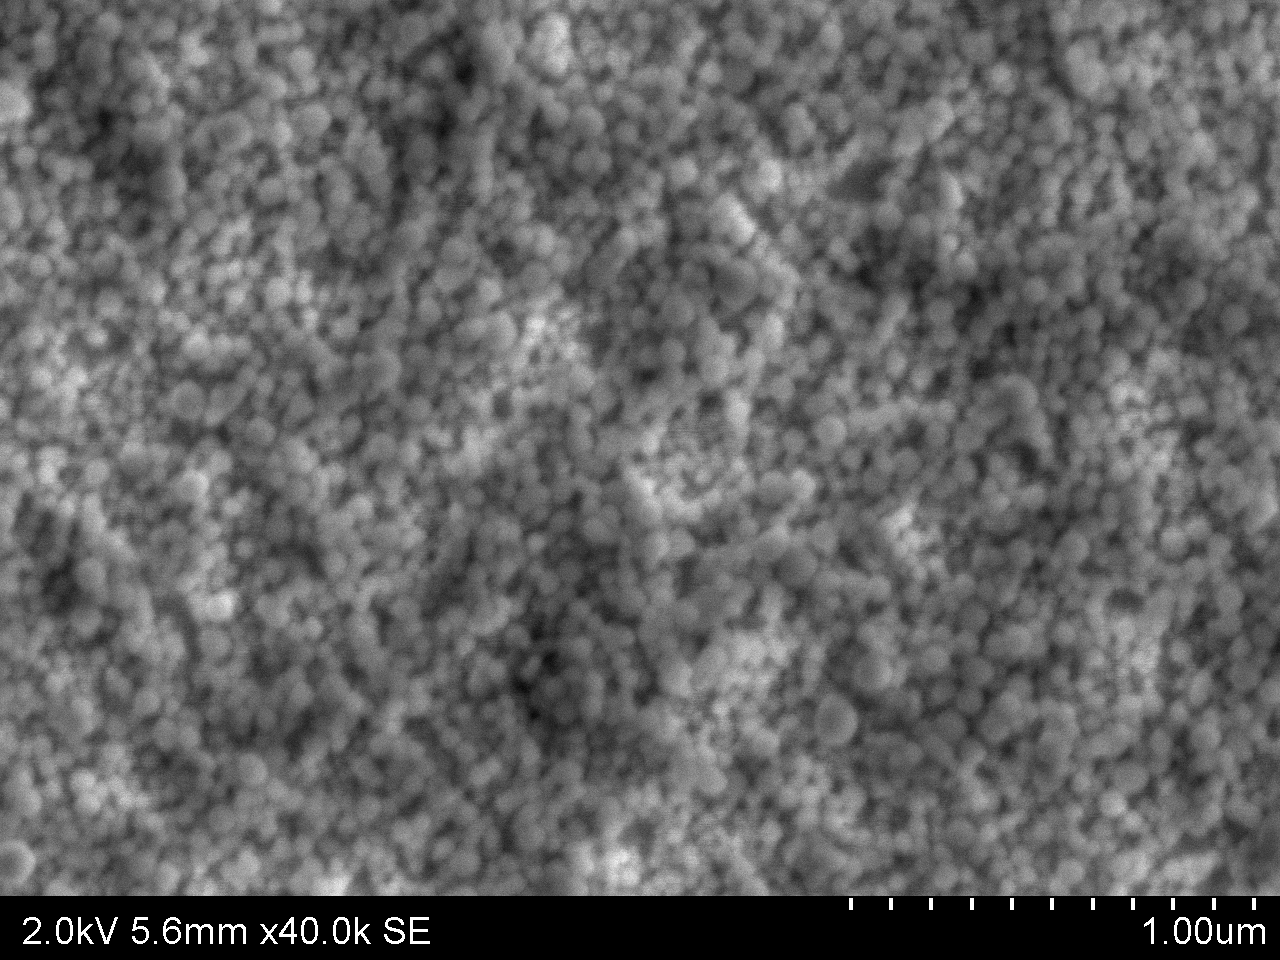
\includegraphics[width=0.8\linewidth]{subAb_sem_03_m006.png}
    \caption[\Ac{sem} image of large silica agglomeration.]{\Ac{sem} image of large agglomeration of particles consisting of silica (\ce{SiO2}).}\label{fig:subAb_silica2_magnified}
\end{figure}

\subsubsection{Stain and particle based on bromine, oxygen and carbon}

Fig.~\ref{fig:subAb_br-stain} shows a stain that consists of bromine, carbon, and oxygen. This type of stain was mainly observed  near the edges of substrate A. The stains were typically \SI{\sim10}{\micro\metre} long. Another type of particle showing the same composition in the \ac{eds} spectrum as the stain was found around the edges as well, see Fig.~\ref{fig:subAb_br-particle}. This particle was typically \SIrange{20}{30}{\micro\metre} long.

%%=========================================
%\section{AFM Study of Etched Substrate A}
\subsection{Surface Roughness}

The \ce{Br}:methanol etched substrate A was characterised for surface topography by \ac{afm}. Images of $\SI{5}{\micro\metre}\times\SI{5}{\micro\metre}$ areas were taken at three different locations on the surface of the substrate: near the centre, upper edge, and upper left corner, as seen in Fig.~\ref{fig:subAb_afm}. The \ac{rms} roughness was calculated to be \SI{0.51}{\nano\metre}, \SI{1.3}{\nano\metre}, and \SI{1.9}{\nano\metre}, respectively, using Eq.~\ref{eq:rmsroughness}. This was an increase in roughness by 2 near the centre, 4 near the edge, and 6 near the corner. The centre had a flat surface with particles with size between \SIrange{10}{50}{\nano\metre} on top, while the edge and corner had a pebbled surface, which made it difficult to see the presence of particles, as seen in Fig.~\ref{fig:subAb_afm_edge}--\oldsubref{fig:subAb_afm_corner}. The surface scratches from before the etch had disappeared, but the presence of polishing particles had increased the roughness of the surface.

\begin{figure}[htbp]
    \centering
    \begin{subfigure}[c]{0.032\linewidth}
        \label{fig:subAb_afm_scale}\captionsetup{list=no}
        
\includegraphics[width=\linewidth]{subAb_afm_scale.png}
    \end{subfigure}
    \hfill
    \mySubfigure{0.3\linewidth}{subAb_afm_centre.png}[fig:subAb_afm_centre] %\SI{0.85}{\nano\metre}
    \hfill
    \mySubfigure{0.3\linewidth}{subAb_afm_upperedge.png}[fig:subAb_afm_edge] %\SI{0.77}{\nano\metre}}
    \hfill
    \mySubfigure{0.3\linewidth}{subAb_afm_upperleftcorner.png}[fig:subAb_afm_corner]%\SI{1,04}{\nano\metre}
    \caption[\Ac{afm} of substrate A after a \ce{Br}:methanol etch.]{\Ac{afm} measurements of substrate A after a \ce{Br}:methanol etch. Images of $\SI{5}{\micro\metre}\times\SI{5}{\micro\metre}$ areas are taken at three different locations on the substrate surface: \subref{fig:subAb_afm_centre} near the centre, \ac{rms} roughness \SI{0.51}{\nano\metre}; \subref{fig:subAb_afm_edge} near the upper edge, \ac{rms} roughness \SI{1.3}{\nano\metre}; and \subref{fig:subAb_afm_corner} near the upper left corner, \ac{rms} roughness \SI{1.9}{\nano\metre}.}\label{fig:subAb_afm}
\end{figure} % AFM, substrate A, with surface pre-growth preparation.

%%=========================================
\subsection{Impurity Analysis -- EDS}
\Ac{eds} was used to get a quantitative analysis of the chemical composition of substrate A after a \ce{Br}:methanol etch. The results can be seen in Table~\ref{tab:subAb_eds_analysis}. The same elements as before the etch were identified. The relative concentrations of \ce{Cd}, \ce{Zn}, and \ce{Te} had an error of less than one percentage point from the expected value of \SI{48}{\atomic\percent} cadmium, \SI{2}{\atomic\percent} zinc, and \SI{50}{\atomic\percent} tellurium. The atomic concentration of alumina was two times as large close to the corner as it was near the edge and centre of the substrate, which was the case even before etch. In addition, the atomic concentration of oxygen was not high enough to be contributing to \ce{Al2O3} and \ce{SiO2} for all the detected aluminium and silicon. This could be due to the overlapping peak of the \ce{O}-K$\alpha$ and \ce{Te}-M lines increasing the uncertainty of the elemental
quantification. A less likely explanation would be that the substrate had inherent aluminium or silicon contamination as well as polishing grit.

\begin{table}[htbp]
    \centering
    \caption[\Ac{eds} impurity analysis of substrate A after a \ce{Br}:methanol etch.]{Results of the \ac{eds} impurity analysis at three different locations on the $\SI{30}{\milli\metre}\times\SI{30}{\milli\metre}$ (111)B \ac{czt} substrate A after a \ce{Br}:methanol etch (atomic concentration \%). The X-ray signal was acquired from $\SI{1270}{\micro\metre}\times\SI{890}{\micro\metre}$ areas near the centre, upper edge, and upper left corner.}\label{tab:subAb_eds_analysis}
   \begin{tabu} to 1.0\textwidth { X[1.85, r] X[1.125,c] X[1.125,c] X[1.125,c] X[1.125,c] X[1.125,c] X[1.125,c] X[1.125,c] } % X[1,c] X[1,c]
        \hline
            & \textbf{\ce{Te}} (at.\%) & \textbf{\ce{Cd}} (at.\%) & \textbf{\ce{Zn}} (at.\%) & \textbf{\ce{Al} } (at.\%) & \textbf{\ce{Si}} (at.\%) & \textbf{\ce{C}} (at.\%) & \textbf{\ce{O}} (at.\%) \\ % \textbf{$X$} (\SI{}{\milli\metre}) &  \textbf{$Y$} (\SI{}{\milli\metre})
        \hline
        Near centre & \SI{45.42}{} & \SI{44.95}{} & \SI{1.84}{} & \SI{0.22}{} & \SI{0.54}{} & \SI{6.05}{} & \SI{0.97}{} \\ % \SI{15.0}{} & \SI{15.0}{}
        Near edge & \SI{45.41}{} & \SI{45.08}{} & \SI{1.72}{} & \SI{0.25}{} & \SI{0.60}{} & \SI{6.01}{} & \SI{0.95}{} \\ % \SI{15.0}{} & \SI{29.0}{} 
        Near corner & \SI{45.18}{} & \SI{44.79}{} & \SI{1.70}{} & \SI{0.56}{} & \SI{0.63}{} & \SI{6.45}{} & \SI{0.70}{} \\ % \SI{1.0}{}  & \SI{29.0}{}
        \hline
    \end{tabu}
\end{table}
%%=========================================

